\documentclass[]{article}
\usepackage{amssymb}
\usepackage{amsmath}
\usepackage[utf8]{inputenc}
\usepackage{graphicx}
\usepackage{booktabs}
\usepackage{listings}
\usepackage{color}
\usepackage{tabularx}
\usepackage{hyperref}

\definecolor{dkgreen}{rgb}{0,0.6,0}
\definecolor{gray}{rgb}{0.5,0.5,0.5}
\definecolor{mauve}{rgb}{0.58,0,0.82}

\lstset{frame=tb,
	%language=C++,
	aboveskip=3mm,
	belowskip=3mm,
	showstringspaces=false,
	columns=flexible,
	basicstyle={\small\ttfamily},
	numbers=none,
	numberstyle=\tiny\color{gray},
	keywordstyle=\color{blue},
	commentstyle=\color{dkgreen},
	stringstyle=\color{mauve},
	breaklines=false,
	breakatwhitespace=true,
	tabsize=2
}


\title{FYS4150 H20 - Project 5:\\Disease Modelling with Runge-Kutta and\\Monte Carlo Simulations}
\author{Olav Fønstelien}

\begin{document}
\maketitle

\begin{abstract}
%The abstract gives the reader a quick overview of what has been done and the most important results. Try to be to the point and state your main findings. It could be structured as follows 
% - Short introduction to topic and why its important 
% - Introduce a challenge or unresolved issue with the topic (that you will try to solve) 
% - What have you done to solve this 
% - Main Results 
% - The implications

\end{abstract}

\section{Introduction} \label{sec:intro}
%When you write the introduction you could focus on the following aspects
% - Motivate the reader, the first part of the introduction gives always a motivation and tries to give the overarching ideas
% - What I have done
% - The structure of the report, how it is organized etc

RK4 optimal with regards to computations and error.

%\clearpage
\section{Background: The SIRS Model} \label{sec:background-sirs}
%classical; introduce vaccine; introduce vital dynamics
%present R0=a/b and Rt=as/b; controlling a through repression or s through vaccination
%Vaccination rates and dependency i,f
%ratio needed to be vaccinated based on the f>=c(a/b-1) relationship

The classical \textit{SIRS} model describes the spread of disease in a population of size $N$, with the transitions between the classes of \textit{Susceptible}, $S$; \textit{Infectious}, $I$; and \textit{Recovering}, $R$. The possible transitions of an individual is cyclic;
\begin{equation}
	S \rightarrow I \rightarrow R \rightarrow S,
\end{equation}
and hence the name. The rates of the transition $S \rightarrow I$ is dependent of a transition rate $a$, and the chance $S/N \cdot I/N$ that each of two interacting individuals are in the groups $S$ and $I$;
\begin{equation}
	\mathrm{rate}(S \rightarrow I) = asi,
\end{equation}
where we have let $s,i$ denote the ratios of susceptibles and infectous in the population $N$. Similarly, the rates of transitions from class $I$ to $R$, and $R$ to $S$ are given by the recovery rate $b$ and the immunity loss rate $c$. These processes happen spontaneously and need no second individual, such that
\begin{equation}
\begin{aligned}
	\mathrm{rate}(I \rightarrow R) &= bi \\
	\mathrm{rate}(R \rightarrow S) &= cr
\end{aligned} \quad,
\end{equation}
where again $r$ is the ratio of recovering individual in population $N$.

From this we can set up the coupled differential equations which describe the rates of transitions between the classes in the population:
\begin{equation} \label{eq:sirs-classic}
\begin{aligned}
	s' &= \mathrm{rate}(R \rightarrow S) - \mathrm{rate}(S \rightarrow I) = cr - asi \\
	i' &= \mathrm{rate}(S \rightarrow I) - \mathrm{rate}(I \rightarrow R) = asi - bi \\
	r' &= \mathrm{rate}(I \rightarrow R) - \mathrm{rate}(R \rightarrow S) = bi - cr
\end{aligned} \quad .
\end{equation}

The classical SIRS model reaches steady state when $s'=i'=r'=0$. Observing that $S + I + R = N$, we get the steady-state ratios
\begin{equation} \label{eq:sirs-classic-steady}
\begin{aligned}
	s^* &= b/a \\
	i^* &= \frac{1 - b/a}{1 + b/c} \\
	r^* &= 1 - s^* - i^* \\
\end{aligned} \quad .
\end{equation}
Here we note that for a disease requires that $i^* > 0$ for it to be able to establish itself within a population, meaning that the steady-state ratio of susceptibles $s^* = b/a < 1$. This ratio is otherwise known as the basic reproduction number $R_0$, defined as the rate of reproduction in a perfectly susceptible population -- that is; a population where $s = 1$, except for the initial infected individual. At a later stage, $s < 1$, and the general reproduction number $R_t$ is given by $as/b$;
\begin{equation} \label{eq:reproduction-numbers}
\begin{aligned}
	R_0 &= b/a \\
	R_t &= as/b \\
\end{aligned} \quad .
\end{equation}
See \cite{milligan2015}.

During the outbreak of disease -- be it the annual influenza or the black plague -- governments and individuals will try to reduce $R_t$ as far as possible or practicable. This can be done only by suppression, i.e. reducing the transmission rate $a$, since as long as the disease exists, $s^* = b/a$, as we will see next. 

If we denote the rate of vaccination within a population $f$, and limit vaccination to those in the $S$ class only, we can describe the rate transition into $R$ from $S$ as
\begin{equation}
	\mathrm{rate}(S \rightarrow R) = fs.
\end{equation}
Introducing vaccination into Equation (\ref{eq:sirs-classic}) gives us
\begin{equation} \label{eq:sirs-vaccinated}
\begin{aligned}
	s' &= cr - asi - fs \\
	i' &= asi - bi \\
	r' &= bi - cr + fs
\end{aligned} \quad .
\end{equation}
Likewise, the steady-state ratios from Equation (\ref{eq:sirs-classic-steady}) now become
\begin{equation} \label{eq:sirs-vaccinated-steady}
\begin{aligned}
	s^* &= b/a \\
	i^* &= \frac{1 - b/a(1 + f/c)}{1 + b/c} \\
	r^* &= 1 - s^* - i^* \\
\end{aligned} \quad ,
\end{equation}
where we again note that a disease needs $b/a < 1$ in order to establish itself, but given a vaccine, the new steady-state ratio is reduced due to the $f/c$ term in $i^*$.

Given a disease with know transmission and immunity loss rates, we may predict the needed rate of vaccination $f$ in order to remove the disease from the population -- that is; $\mathrm{argmin}_{f} i^*(f) = 0$. From Equation (\ref{eq:sirs-vaccinated-steady}) we see that $f = c(a/b - 1) - i^*a(c/b + 1)$, and $i^* = 0$ is thus achieved when
\begin{equation} \label{eq:vaccination-rate-min}
	f \ge c(a/b - 1).
\end{equation}
Likewise, by setting $i = 0$ in Equation (\ref{eq:sirs-vaccinated-steady}) we find how large part of the population to vaccinate -- or rather; how large part of the population which has to have antibodies against a pathogen as $i \rightarrow i^* = 0$:
\begin{equation} \label{eq:vaccination-fraction}
	r \rightarrow r^* = 1 - \frac{1}{1 + f/c}.
\end{equation}
Thus, only after the disease has been eradicated does the $s^* = b/a$ relationship cease to exist. $s^*$ is then given as
\begin{equation}
	s^* = \frac{1}{1 + f/c}.
\end{equation}

At last, we may also introduce vital dynamics -- births and deaths -- into the SIRS model to be able to study the effect of deadly diseases over longer periods of time. Given a birth rate $e$, a background death rate $d$ and a the incidence death rate $d_I$, the full form of the SIRS model becomes
\begin{equation} \label{eq:sirs-vitals}
\begin{aligned}
	s' &= cr - asi - fs - ds + e \\
	i' &= asi - bi - di -d_Ii\\
	r' &= bi - cr + fs - dr
\end{aligned} \quad ,
\end{equation}
where we have assumed that newborns are initially susceptible. The steady-state ratios $s^*, i^*, r^*$ are more complicated to attain, and in this report we will find these with the help of the numerical models which we will developed in the following chapter. This will allow us to introduce time-varying rates, such as transmission rates affected by government policy, or delayed availability of vaccines. 

%\clearpage
\section{Methods} \label{sec:methods}
% - Describe the methods and algorithms
% - You need to explain how you implemented the methods and also say something about the structure of your algorithm and present some parts of your code
% - You should plug in some calculations to demonstrate your code, such as selected runs used to validate and verify your results. The latter is extremely important!! A reader needs to understand that your code reproduces selected benchmarks and reproduces previous results, either numerical and/or well-known closed form expressions.

The differential equation for the SIRS model as stated in Equations (\ref{eq:sirs-classic}), (\ref{eq:sirs-vaccinated}), (\ref{eq:sirs-vitals}) does not have an analytical solution. In this chapter we will develop two algorithms for solving them; one based on the Fourth order Runge-Kutta numerical method; and one based on Monte Carlo simulation.

\subsection{Fourth Order Runge-Kutta Algorithm for the SIRS Model} \label{sec:runge-kutta}
The Fourth Order Runge-Kutta method, or simply RK4, is based on \textit{Simpson's Rule} for numerical integration, by which
\begin{equation} \label{eq:simpsons-rule}
	\int_{a}^{b} f(x) dx = \frac{1}{6} \big( f(a) + 4f((b+a)/2) + f(b) \big) + O(h^5),
\end{equation}
-- that is; an approximation of $f$'s slope over $[a,b]$ by the weighted function values at the end points $a,b$ and the midpoint $(a+b)/2$.

Given a first-order differential equation on the form
\begin{equation}
	\frac{dy}{dt} = f(t, y),
\end{equation}
we can approximate $y(t)$ numerically by $y_t$ as
\begin{equation}
\begin{aligned} \label{eq:re4-1st-step}
		y_{i+1} &= y_i + \int_{t_i}^{t_{i+1}} f(t,y) dt \\
		&= \frac{h}{6} \big( f(t_i, y_i) + 4f(t_{i+1/2}, y_{i+1/2}) + f(t_{i+1}, y_{i+1}) \big) + O(h^5)
\end{aligned} \quad ,
\end{equation}
where $h=t_{i+1} - t_i$ is the step size. The midpoint and endpoint values $y_{i+1/2}$ and $y_{i+1}$ are unknown to us. We may approximate $y_{i+1/2}$ as $y^*_{i+1/2}$ by \textit{Euler's Forward Method} with step size $h/2$ such that
\begin{equation}
	y_{i+1/2} = y_i + \frac{h}{2} f(t_i, y_i) + O(h^2) \Rightarrow y^*_{i+1/2} = y_i + \frac{h}{2} f(t_i, y_i),
\end{equation}
but instead of applying this directly into Equation (\ref{eq:re4-1st-step}), RK4 now splits the middle term in two;
\begin{equation}
	4f(t_{i+1/2}, y_{i+1/2}) \rightarrow 2f(t_{i+1/2}, y^{*}_{i+1/2}) + 2f(t_{i+1/2}, y^{**}_{i+1/2}),
\end{equation}
where $y^{**}_{i+1/2}$ in the second term is an improved approximation of $y_{i+1/2}$ using
\begin{equation}
	y^{**}_{i+1/2} = y_i + \frac{h}{2} f(t_{i+1/2}, y^{*}_{i+1/2}).
\end{equation}
Following the same pattern, $y_{i+1}$ in the last term is approximated by $y^*_{i+1}$ using $y^{**}_{i+1/2}$ such that
\begin{equation}
	y^{*}_{i+1} = y_i + h f(t_{i+1/2}, y^{**}_{i+1/2}).
\end{equation}
We end up with an approximation $y^{**}_{i+1}$ which is given by
\begin{equation}
	y^{**}_{i+1} = y_i + \frac{h}{6} \big( f(t_i, y_i) + 2f(t_i + \frac{h}{2}, y^*_{i+1/2}) + 2f(t_i + \frac{h}{2}, y^{**}_{i+1/2}) + f(t_i+h, y^*_{i+1}) \big).
\end{equation}
The error is similar to that of Simpson's Rule, $O(h^5)$, which adds up to $O(h^4)$ over the whole run from $t_1=t_0+h$ to $t_n=t_0+nh$. This comes however at the cost of seven evaluations of $f(t,y)$ at each time step, compared with only one for Euler's method, which again has an overall error $O(h)$.

Algorithmically, the steps are given in Listing \ref{lst:rk4-steps} and is very simple to implement. It runs in $\mathcal{O}(n)$ time and requires no memory of the earlier calculation steps. It is CPU-bound.

\begin{lstlisting}[caption={Fourth order Runge-Kutta algorithm.},label={lst:rk4-steps},escapeinside={@}{@}] [!h]
ALGORITHM RUNGE-KUTTA(f, ti, yi, h)
	Inputs: function f, time ti, value yi at time ti, step size h.
	Outputs: approximation of y at time ti+h.
	
	k1 = h*f(ti, yi)
	k2 = h*f(ti+h/2, yi+k1/2)
	k3 = h*f(ti+h/2, yi+k2/2)
	k4 = h*f(ti+h, yi+k3)
	OUTPUT yi + (k1 + 2*k2 + 2*k3 + k4)/6

END ALGORITHM
\end{lstlisting}

The SIRS model as described in Equation (\ref{eq:sirs-vitals}) can be implemented directly as it stands using the Runge-Kutta algorithm in Listing \ref{lst:rk4-steps}. We will however add an equation for the population growth rate $n'$, giving the following set of equations;

\begin{equation} \label{eq:sirs-rk4}
\begin{aligned}
	s' &= cr - asi - fs - ds + e \\
	i' &= asi - bi - di -d_Ii \\
	r' &= bi - cr + fs - dr \\
	n' &= e - d - id_I
\end{aligned} \quad .
\end{equation}

We must select a suitable time step $h$, and update all approximations for each iterations, using only the values from the earlier iteration. However, we might update the last equation, say that for $r_i$ based on the results of the others, since $r_i = n_i - s_i - i_i$ at all times. This improves numerical stability. A possible implementation is outlined in Listing \ref{lst:rk4-sirs}.

\begin{lstlisting}[caption={SIRS model Runge-Kutta algorithm.},label={lst:rk4-sirs},escapeinside={@}{@}] [!h]
ALGORITHM SIRS-RUNGE-KUTTA(fs, fi, fn, t0, s0, i0, n0, n, h)
	Inputs: functions fi, fi, fn, initial time t0, 
			initial values s0, i0, n0, time steps n, step size h.
	Outputs: approximation of s, i, r, n at time
			 t=t0+h, t0+2*h, ..., t0+n*h
	
	s = s0
	i = i0
	n = n0
	t = t0
	FOR k IN 1...n DO
		s = RUNGE-KUTTA(fs, t, s, h)
		i = RUNGE-KUTTA(fi, t, i, h)
		n = RUNGE-KUTTA(fn, t, n, h)
		r = n - s - i
		t = t + h
		OUTPUT s, i, r, n
	END FOR

END ALGORITHM
\end{lstlisting}

Possible extensions to the Fourth Order Runge-Kutta algorithm include the \textit{Runge-Kutta-Fehlberg} algorithm, which applies adaptive time step for error control and optimalization. See \cite{fys4150-notes} for more on this issue as well as numerical methods for solving differential equations in general.

\subsection{Monte Carlo Algorithm for the SIRS Model} \label{sec:monte-carlo}
%lets us calculate discrete values
The Runge-Kutta method inherently implicates continuous values for the ratios of susceptibles $s$, infectious $i$, and recovering $r$ in the population. The Monte Carlo method, on the other hand, lets us calculate the discrete changes in each class, and thereby simulate a possible trajectory for the spread of the disease and the effect it has on the population. 

Before we run the simulation, however, the expectation value at each step in the trajectory is exactly the solution to the differential equation describing the SIRS model;
\begin{equation}
	\mathbb{E}(y_i) = y(t_i)
\end{equation}
The Monte Carlo method will therefore give us an estimate $\bar{\mu}_i$ of the solution if we calculate its mean value. The estimate follows the $t$-distribution and if we run $n$ simulations it has standard deviation $\bar{\sigma}_i$ given by
\begin{equation}
	\bar{\sigma}_i^2 = \frac{1}{n-1} \sum_{j=1}^{n} (y_j - \bar{\mu}_i)^2.
\end{equation}
From this we can calculate a confidence interval for the \textit{true} $\mu_i = y(t_i)$, i.e. the solution to the equations. A $100 \cdot (1-\alpha)$ \% confidence interval is given by
\begin{equation}
	\bar{\mu}_i - t_{\alpha/2, \nu} \frac{\sigma}{\sqrt{n}} < y(t_i) < \bar{\mu}_i + t_{\alpha/2, \nu} \frac{\sigma}{\sqrt{n}},
\end{equation}
where $\nu = n-1$ denotes the $t$-distribution's degrees of freedom. See \cite{devore2012}. As $\nu \rightarrow \infty$, the $t$-distribution converges towards the normal distribution, but for small $n$, i.e in the 10's or 20's, it does matter. A CI$_{90}$ has a multiplier of 1.64 for the normal distribution, while it is 1.83 for the $t$-distribution with $\nu=9$. Corresponding values for CI$_{99}$ are 2.58 and 3.25.

We implement the Monte Carlo method by first discretizing the SIRS model in Equation (\ref{eq:sirs-vitals});
\begin{equation} \label{eq:sirs-vitals-discrete}
\begin{aligned}
	S' &= cR - \frac{aSI}{N} - fS - dS + eN \\
	I' &= \frac{aSI}{N} - bI - dI -d_II\\
	R' &= bI - cR + fS - dR
\end{aligned} \quad ,
\end{equation}
where we have let the upper-case letters $S,I,R,N$ denote discrete variables and their derivatives. Next, we translate the transition rates $\mathrm{rate}(X \rightarrow Y)$ into probabilities that a transition will happen within a time step $\Delta t$ of our simulation;
\begin{equation} \label{eq:transition-probabilities}
\begin{aligned}
	P(S \rightarrow I) &= \frac{aSI}{N} \Delta t \\
	P(S \rightarrow R) &= fS \Delta t \\
	P(S \rightarrow D) &= dS \Delta t \\	
	P(B \rightarrow S) &= eN \Delta t \\	
	P(I \rightarrow R) &= bI \Delta t \\	
	P(I \rightarrow D) &= dI \Delta t \\	
	P(I \rightarrow D_I) &= d_II \Delta t \\	
	P(R \rightarrow S) &= cR \Delta t \\	
	P(R \rightarrow D) &= dR \Delta t \\		
\end{aligned} \quad .
\end{equation}
Here, we have let $D$ denote deaths from other causes than the disease; $D_I$ deaths from the disease; and $B$ denote births, which again are all assumed into class $S$, i.e. susceptible. Since we cannot have any half deaths or half births, and since at any point in the simulation do not know the development in the next steps, we must adapt $\Delta t$ such that at any time at most one individual is likely to transition from one class to another. To find $\Delta t$, observe that for all but the new infections, the highest probability for the transition out of one class $X$ into another class $Y$ occurs when all $N$ individuals are in $X$. For new infections we have the highest rate when exactly half of the population are in each class $S,I$. Consequently, the time step $\Delta t$ must satisfy
\begin{equation}
\begin{aligned}
	\mathrm{argmax}_X  P(X \rightarrow Y) &= qN \Delta t \le 1 \\
	\mathrm{argmax}_{S,I} P(S \rightarrow I) &= \frac{aN}{4} \Delta t \le 1
\end{aligned} \quad .
\end{equation}
For remembering that we may also have time-varying transition rates, such as seasonal vaccination or policy-suppressed transmission rates, we must adapt the time step at each iteration in the simulation such that
\begin{equation} \label{eq:dt-min}
	\Delta t = \frac{1}{N} \cdot \mathrm{min} \bigg( \frac{4}{a}, \frac{1}{b}, \frac{1}{c}, \frac{1}{d}, \frac{1}{d_I}, \frac{1}{e}, \frac{1}{f} \bigg).
\end{equation}

Now, having decided on the time step for iteration $i$, say, we draw a random number $\varepsilon_i \sim \mathcal{U}(0,1)$, and transition one individual from class $X$ to $Y$ if $\varepsilon_i < P_i(X \rightarrow Y)$. Since all transitions \textit{within one iteration} of the simulation are independent, we may reuse $\varepsilon_i$ when we do all the transition tests in that iteration. 

An outline of the resulting SIRS model Monte Carlo algorithm if given in Listing \ref{lst:mc-sirs}. As for the Runge-Kutta algorithm in Listing \ref{lst:rk4-sirs} we update \lstinline|R| by summing over the other classes, both for simplicity and for numerical stability.

\begin{lstlisting}[caption={SIRS model Monte Carlo algorithm.},label={lst:mc-sirs},escapeinside={@}{@}] [!h]
ALGORITHM SIRS-MONTE-CARLO()
	Inputs: initial population distribution S0, I0, R0, N0,
	time-varying transition rates a, b, c, d, dI, e, f,
	initial time t0, end time tn.
	Outputs: approximation of S, I, R, N at time
	t1=t0+dt1, t2=t0+dt2, ..., tn.
	
	S = S0
	I = I0
	R = R0
	N = N0
	t = t0
	WHILE t <= tn DO
		dt = get_time_step(N, t)  // (@Equation (\ref{eq:dt-min})@)
		epsilon = draw_random_number()
		{collect incremental transitions from 
		 all combinations in @Equation (\ref{eq:transition-probabilities})@.
		 Make all transitions where probability < epsilon}
		S = S + {transitions into class S}
		I = I + {transitions into class I}
		N = N + {sum of births and deaths}
		R = N - S - I
		
		OUTPUT S, I, R, N, t
		t = t + dt
	END WHILE

END ALGORITHM
\end{lstlisting}


%\clearpage
\section{Results} \label{sec:results}
% - Present your results
% - Give a critical discussion of your work and place it in the correct context.
% - Relate your work to other calculations/studies
% - An eventual reader should be able to reproduce your calculations if she/he wants to do so. All input variables should be properly explained.
% - Make sure that figures and tables should contain enough information in their captions, axis labels etc so that an eventual reader can gain a first impression of your work by studying figures and tables only.

We will now go through the results and see how our two numerical models perform. We will in all cases see corresponding results for both models. 

The results are structured in the order of increasing complexity. We begin in Section \ref{sec:recovery-rates} by examining the importance of the ratio of the recovery and transmission rates in the establishment of a disease within a population. We saw this as the basic reproduction number $R_0$ in Section \ref{sec:background-sirs}. After looking at these static conditions, we will see how seasonal variations affects the dynamics of the disease over the year.

In Section \ref{sec:vaccines} we will introduce the effect of a vaccine and further study its effect on the spread of a disease. We will see how the vaccination rate must be adjusted for the disease to gradually disappear, or even be kept at a constant level within the population, which is the case with many diseases. We will introduce seasonal variations here as well, and see how the dynamics that this introduces very much resembles the seasonal transmission rate variations.

After that, in Section \ref{sec:vital-dynamics}, we will perform a longer simulation to see how infection levels of a deadly disease affects the long-term growth of a population with a fixed birth and background death rate.

At last we will bring it all together when we try to reproduce the 2020 SARS-CoV-2 pandemic, with corresponding government policies, transmission rate seasonality and -- looking into the future -- finally the advent of a vaccine.

Note that unless otherwise is stated, the disease parameters for transmission rate, recovery rate and immunity loss rate can be assumed to be $a=4, b=1, c=0.5$. For the Monte Carlo simulations, population size can be assumed to be $N=400$ and initial number of infectious individuals $I=100$.

\subsection{The Importance of $R_0$} \label{sec:recovery-rates}
%Show development for various ratios; tie this to R0=a/b and Rt=as/b, also with regards to controlling a through repression or s through vaccination
%present distributions 5<t<10000
%Include seasonal variations

As we saw in Section \ref{sec:background-sirs}, Equation (\ref{eq:reproduction-numbers}), success or failure on a infectious disease's term depends on its basic reproduction number $R_0$, which is given by its recovery vs. transmission ratio $a/b$. Figure \ref{fig:recovery-transmission-ratio} shows Runge-Kutta (RK4) and Monte Carlo (MC) simulations for four different ratios at constant immunity loss rate $c$. We see that gradually increasing the recovery rate also gradually decreases the steady-state infectious fraction $i^*$, as we would expect from Equation (\ref{eq:sirs-classic-steady});
\begin{equation}
	i^* = \frac{1 - b/4}{1 + 2b}.
\end{equation}
For $b = 1$, the disease establishes itself in 25 \% of the population at any given time; doubling the recovery rate reduces this to 10 \%. At $b = 3$, a mere 3.5 \% remain infected, while at $b = 4$, corresponding to exactly $i^* = 0$, the disease gradually disappears without ever getting a foothold.

\begin{figure}[!h]
	\centering
	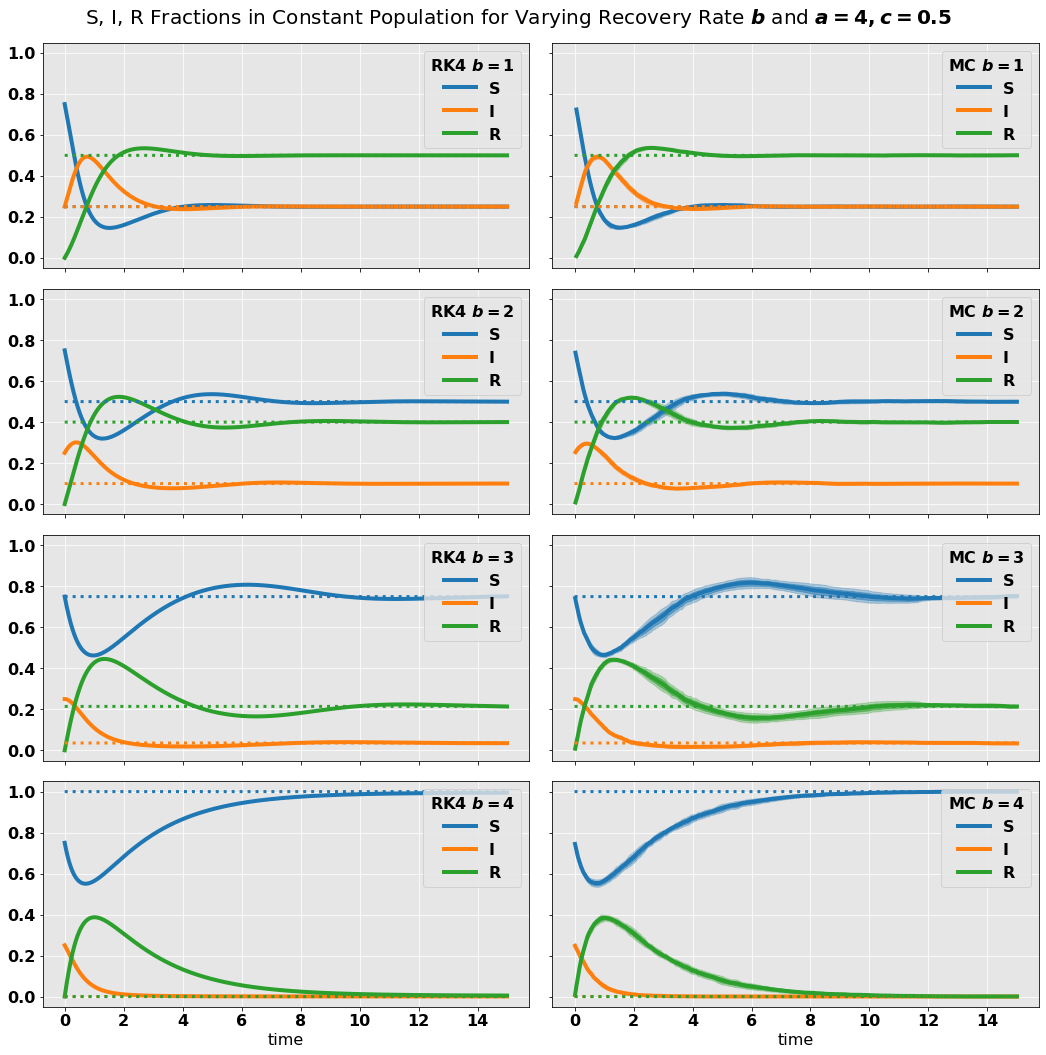
\includegraphics[width=1\linewidth]{./figs/recovery-transmission-ratio.png}
	\caption{Runge-Kutta (RK4) simulations in the left column and Monte Carlo (MC) in the right for a population of size 400 with initially 100 infected individuals. Results from both algorithms largely overlap and converge towards the expected values (dotted same color). MCs are mean of 10 simulations with CI$_{99}$ bands indicated as same-color shades. We see that the CI band is wider for the areas with high dynamic.}
	\label{fig:recovery-transmission-ratio}
\end{figure}

With only 400 individuals in the population simulated by the MC algorithm in Figure \ref{fig:recovery-transmission-ratio}, the system still seems very deterministic. We see that only in the most dynamical periods do we have a noticeable shade around the curves, denoting the CI$_{99}$ interval. This impression is also largely confirmed when we look at Figure \ref{fig:recovery-transmission-ratio-distribution}. We see the distribution for each of the curves $S, I, R$ in the $b=3$ case, sampled since steady-state at $t=10$ until $t=10^4$. The distribution more closely resemble the anticipated normal distribution for all populations, but the distribution is markedly sharper for $I$. This is given by Equation (\ref{eq:transition-probabilities}) in that a deviation from the expectation value $\mu$ has a more forceful pull back towards $\mu$ for $I$ than for the other. From Equation (\ref{eq:dt-min}) we see that $a=4, b=3, c=0.5$ give the transition probability deltas
\begin{equation}
\begin{aligned}
	\Delta P(S \rightarrow I) &= \frac{3 \cdot (299 \cdot 15 - 300 \cdot 14)}{400} \cdot \Delta t = 2.1375 \Delta t \\		
	\Delta P(I \rightarrow R) &= 3 \cdot (13 - 14) \Delta t = - 3\Delta t \\	
	\Delta P(R \rightarrow S) &= 0.5 \cdot (85-86) \Delta t = - 0.5\Delta t \\		
\end{aligned} \quad .
\end{equation}
Consequently, we will have a larger variation in $S$ and $R$ populations, while any deviation from the expectation value in the $I$ population will quickly be sent on to $R$. We should also expect that the distribution for $I$ is a little shifted upwards, which is also what we see in the figure.

\begin{figure}[!h]
	\centering
	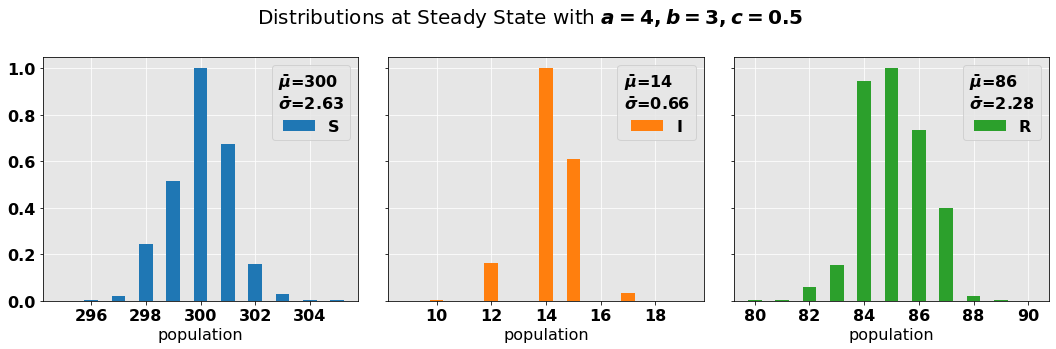
\includegraphics[width=1\linewidth]{./figs/recovery-transmission-ratio-distribution.png}
	\caption{Population distribution for steady-state Monte Carlo simulation for the $b=3$ case in Figure \ref{fig:recovery-transmission-ratio}. Population size is 400 and simulation. The distributions largely follow the normal distribution.}
	\label{fig:recovery-transmission-ratio-distribution}
\end{figure}

By introducing seasonality in $a$, we can simulate the dynamics of the disease over the year. In Figure \ref{fig:seasonal-transmission-rate} we see the $b=1$ case from earlier with seasonal transmission rate as the dotted grey line. The rate has a peak at $t=0$, and a period $T=10$. The resulting pattern of infection closely follows the infection rate phase, but the shape is different. Due to the degree of immunity, as well as infection, and hence decrease of available susceptible individuals, the infection curve quickly rises before it slowly decreases and hits the bottom in the middle of the year.

\begin{figure}[!h]
	\centering
	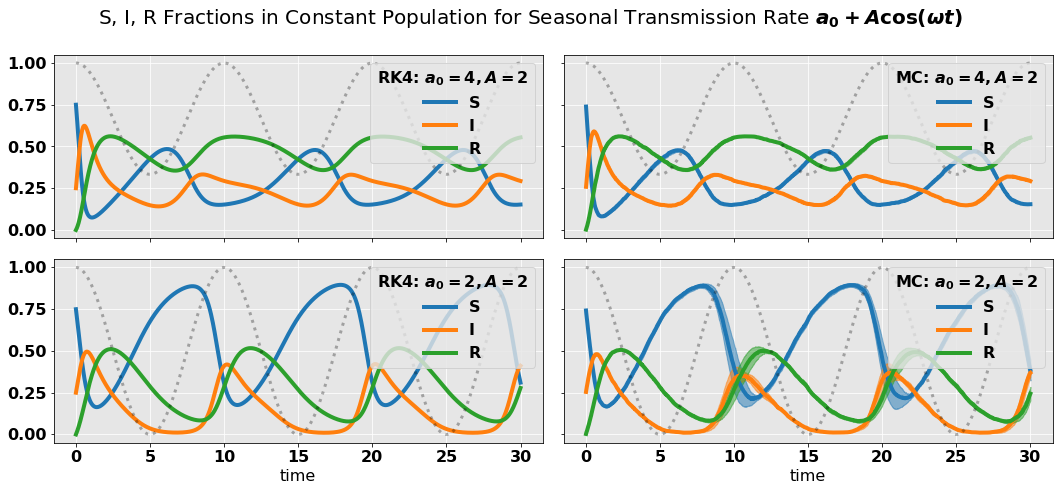
\includegraphics[width=1\linewidth]{./figs/seasonal-transmission-rate.png}
	\caption{RK4 (left) and MC (right) simulation of seasonal variations in the transmission rate with $b=1, c=0.5$. The infection rate curve, shown as a dotted gray line, is closely followed by the infection rate.}
	\label{fig:seasonal-transmission-rate}
\end{figure}


\subsection{Introducing Vaccines} \label{sec:vaccines}
%modelling expected i based on f and vice versa
%ratio needed to be vaccinated based on the f>=c(a/b-1) relationship
%seasonal variations in i even if mean of f = fopt

In Section \ref{sec:background-sirs} we saw that, given a disease with parameters $a,b,c$, the level of infection can be controlled by vaccinating a corresponding portion of the population given by Equation (\ref{eq:vaccination-fraction}). To completely get rid of the disease, we must have a rate of vaccination $f \ge c(a/b - 1)$.

In Figure \ref{fig:vaccination-rates} we see the effect of using vaccines against a disease with parameters $a=4, b=1, c=0.5$. We see that by increasing the level of immunity in the population from 50 \%, which is the level without vaccines, to 65 \% decreases the infection level by the same 15 \% from 25 \% to 10 \%.  Further increasing the immunity to 75 \% removes it all together. Thus, we see that by moving individuals from the $S$ class into $R$ class, we are in reality \textit{removing} them from the $I$ class. This corresponds to what we found in Equation (\ref{eq:sirs-vaccinated-steady}).

\begin{figure}[!h]
	\centering
	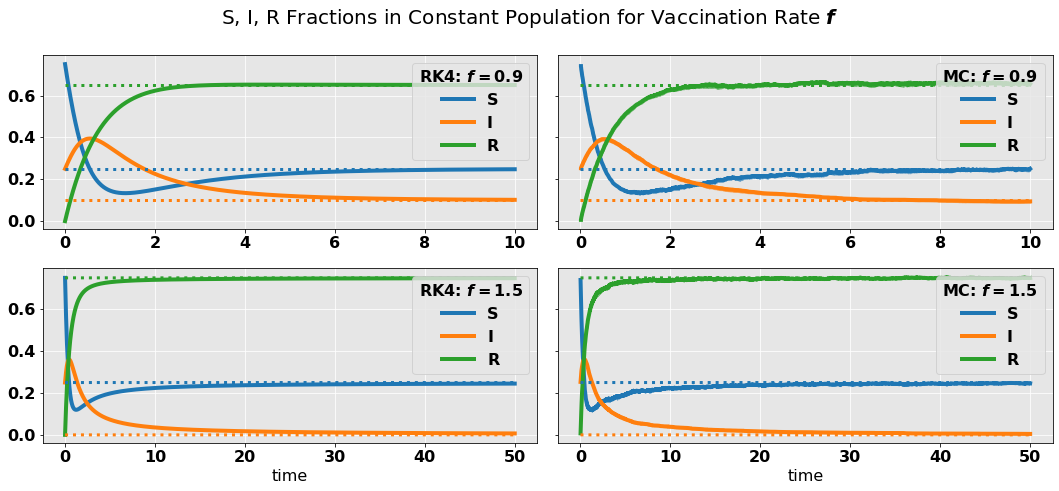
\includegraphics[width=1\linewidth]{./figs/vaccination-rates.png}
	\caption{RK4 (left) and MC (right) simulation of the effect of vaccination in a population. Disease parameters are $a=4, b= 1, c=0.5$, and for MCs, $N=400$. Vaccination removes individuals from the $I$ group.}
	\label{fig:vaccination-rates}
\end{figure}

Similar to what we saw for seasonal variations in the transmission rate in the former section, a seasonal vaccination rate provokes an annual ebb and flow in the infection rates, as we see in Figure \ref{fig:seasonal-vaccination-rate}. We note, however, that even if we on average apply the vaccination rate which would eventually remove the disease in the steady-state case, the disease remains in the seasonal case. 

\begin{figure}[!h]
	\centering
	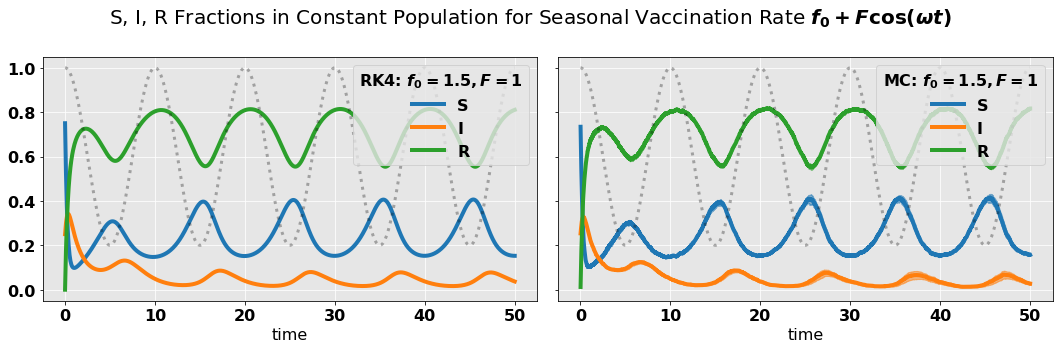
\includegraphics[width=1\linewidth]{./figs/seasonal-vaccination-rate.png}
	\caption{RK4 (left) and MC (right) simulation of the effect of seasonal vaccination in a population. Vaccination rate is indicated by the dotted gray line and has a peak at $t=0$ and period $T=10$. As earlier, disease parameters are $a=4, b= 1, c=0.5$, and for MCs, $N=400$. We see that seasonality in vaccination rates translates into seasonality in infections.}
	\label{fig:seasonal-vaccination-rate}
\end{figure}


\subsection{Introducing Vital Dynamics} \label{sec:vital-dynamics}
%non-deadly; collapse; equilibrium
%ratio reaches equilibrium independently of the d,dI,e ratio
%Monte Carlo is optimistic -- >99% sure about survival; RK4 more pessimistic -- collapse of the population

Let us now study the effect of a disease on the long-term development of the population by introducing an incidence death rate $d_I$ from the disease, along with a background death rate $d$ and birth rate $e$. We assume a constant background death rate $d=0.01$, birth rate $e=0.02$, and a apply different $d_I$ for a disease with otherwise fixed, constant parameters $a=4, b=1, c=0.5$. In Figure \ref{fig:dynamic-pop-infected-ratio} we see that as for the constant population cases in Section \ref{sec:recovery-rates}, the fraction of infectious individuals finds a steady state. The level does not correspond to the levels we saw earlier, though, due to the imbalance introduced by $d, e, d_I$ in the steady-state equations. In the figure we see that the Monte Carlo and Runge-Kutta results correspond quite well, except for the $d_I = 1.00$ case, where Runge-Kutta presents a constant fraction, while Monte Carlo predicts a collapse, and hence eradication of the disease, at around $t=25$. The simulation has been run 30 times, and the CI$_{99}$ follows the mean towards zero.



\begin{figure}[!h]
	\centering
	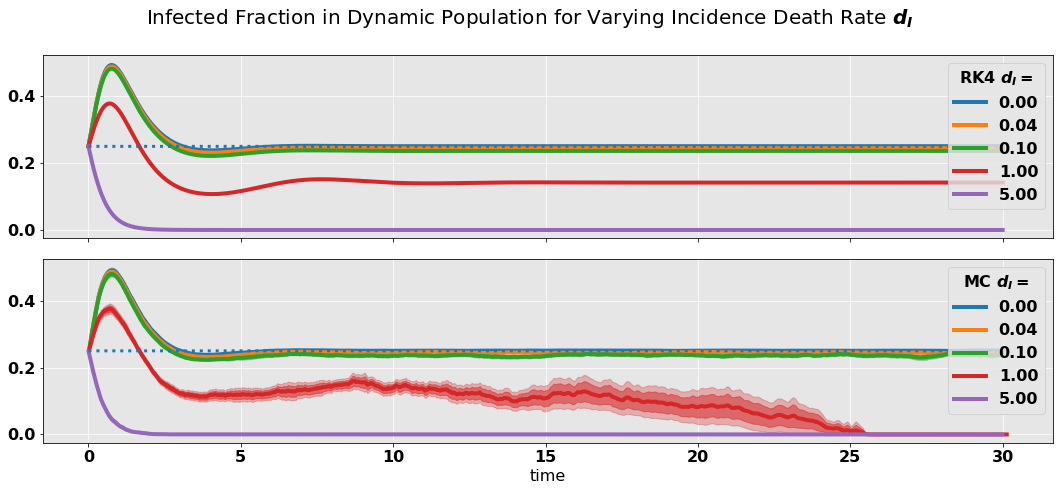
\includegraphics[width=1\linewidth]{./figs/dynamic-pop-infected-ratio.png}
	\caption{RK4 (left) and MC (right) simulation of the effect vital dynamics and incidence death rate $f_I$ on a population. RK4 finds a steady state for any $d_I$, as does MC, with one exception. For $d_I = 1.00$, the RK4 and MC simulations deviate drastically. The explanation is found in Figure \ref{fig:dynamic-pop-pop-growth}.}
	\label{fig:dynamic-pop-infected-ratio}
\end{figure}

The explanation for the collapse in infections predicted by Monte Carlo becomes clear when we look at the development of the populations. In the $d_I=1.00$ case, the population is all but extinguished, and  it in this scenario that Monte Carlo predicts the last infected individual to die, while there still is a small population left which then starts to grow ever so slowly. This outcome is not possible in a Runge-Kutta simulation since the populations are only represented by continuous fractions, which of course may not become zero.

The small population at the end of the $d_I=1.00$ case also explains the high variance in the mean value, since it reflects incremental changes on a small scale.

Another interesting case is the $d_I=5.00$, which represents a disease so deadly that $R_0 < 1$, and hence the disease disappears by itself. For $d_I=0.04$, the population size remains constant, meaning that the birth surplus $e-d = 0.01$ correspond exactly to the deaths $d_Ii = 0.04 \cdot 0.25 = 0.01$.


\begin{figure}[!h]
	\centering
	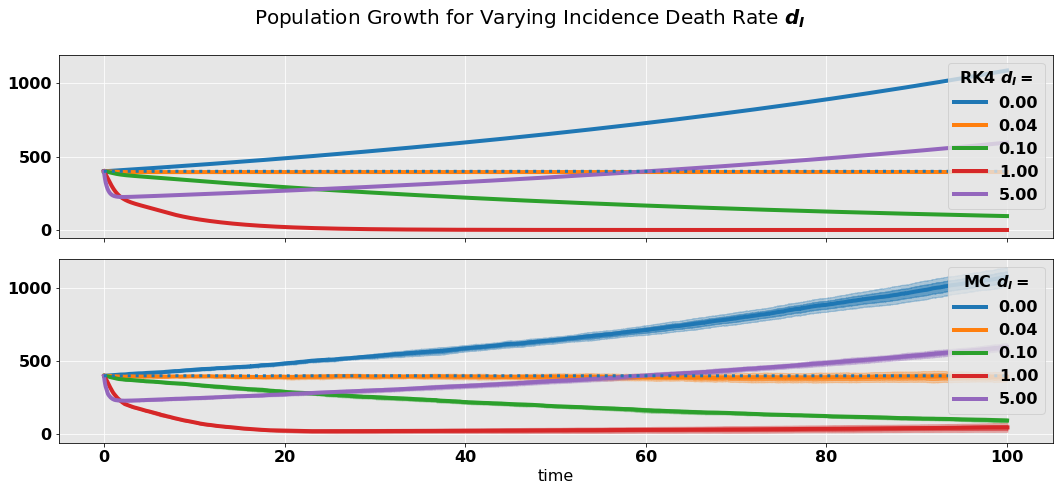
\includegraphics[width=1\linewidth]{./figs/dynamic-pop-pop-growth.png}
	\caption{RK4 (left) and MC (right) simulation of the effect of incidence death rate $d_I$ on the population. Constant population is achieved when $e-d=d_Ii$, as we see for $d_I=0.04$. For $d_I=1.00$, the MC simulations consistently predict eradication of the disease, something which is not possible for RK4.}
	\label{fig:dynamic-pop-pop-growth}
\end{figure}



\subsection{Bringing it All Together: COVID-19 Case Study} \label{sec:case-study}
%policies as bathtub curves
%vaccine availability as exponential curve
%effect of early introduction of lockdown vs strictness

We will now combine what we have learned from looking at the seasonality of vaccines and transmission rates in the above results with government policies and non-availability of vaccines, using COVID-19 as a case study \cite{who-url}. The science on this disease is still uncertain, but we will assume a strong seasonal factor in its transmission rate which peaks at new year; $a(t) = 3 + 2.25 \cos (5\pi t) $. Further, we will assume an influenza-like vaccination seasonality once that gets going, with a peak during the autumn months, such that $f(t) = 1 + 0.5 \cos (5\pi (t+2.5))$. Further, and critically, we will assume government imposed \textit{lockdowns} 


\begin{figure}[!h]
	\centering
	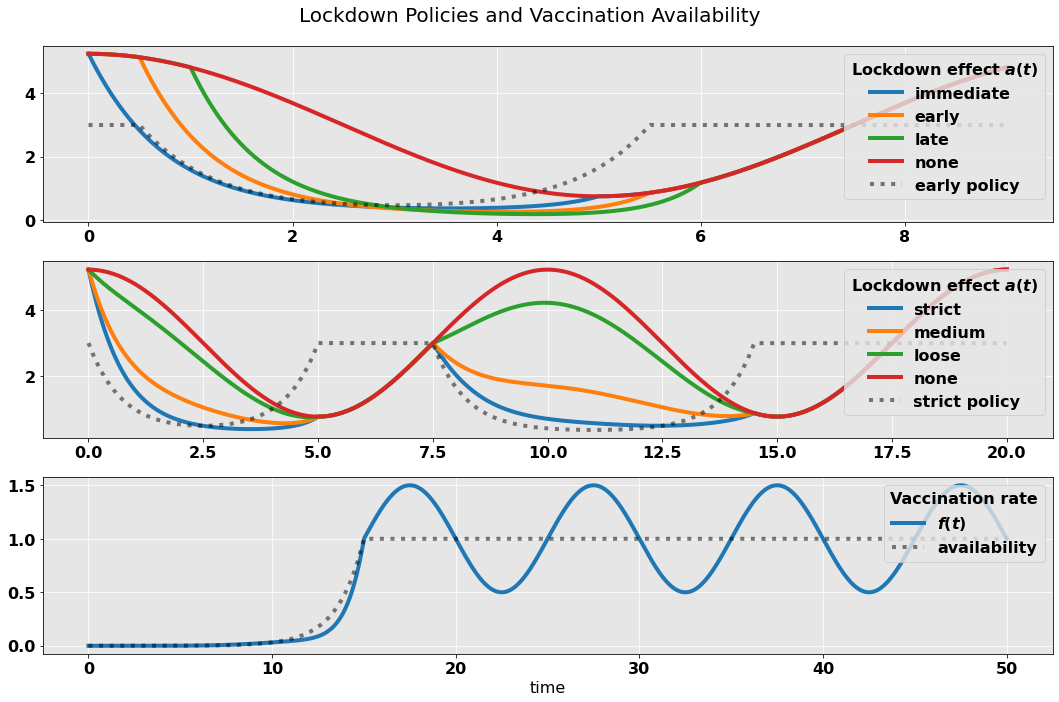
\includegraphics[width=1\linewidth]{./figs/covid-policy.png}
	\caption{}
	\label{fig:covid-policy}
\end{figure}


\begin{figure}[!h]
	\centering
	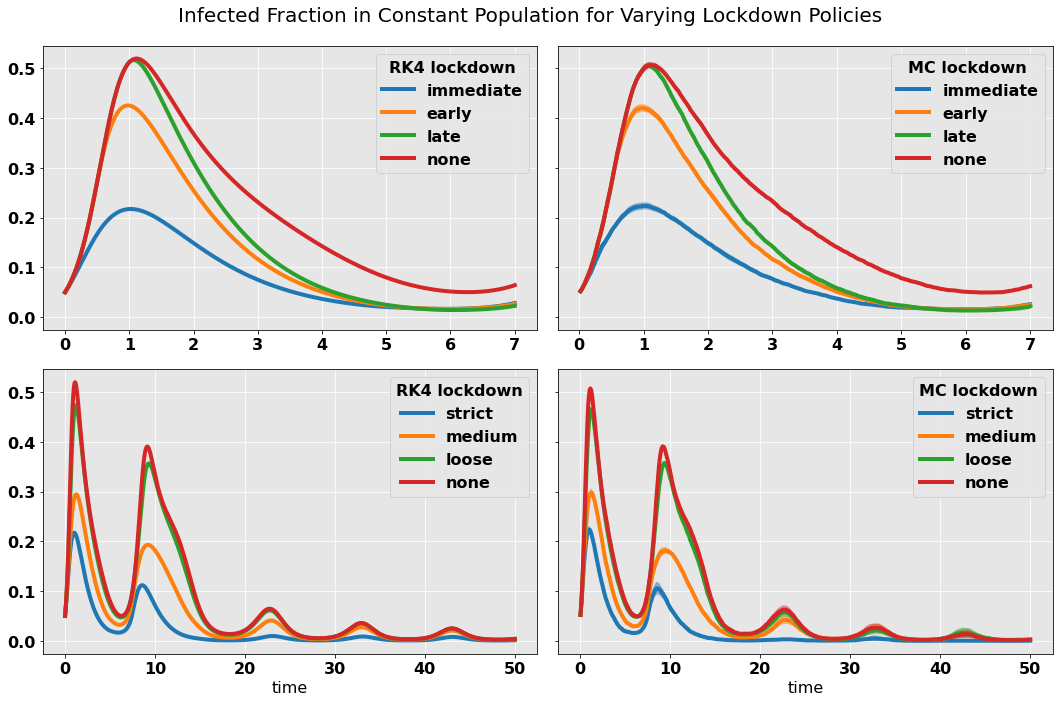
\includegraphics[width=1\linewidth]{./figs/covid-infection-sim.png}
	\caption{}
	\label{fig:covid-infection-sim}
\end{figure}


\clearpage
\section{Discussion and Conclusion} \label{sec:conclusion}
% - State your main findings and interpretations
% - Try as far as possible to present perspectives for future work
% - Try to discuss the pros and cons of the methods and possible improvements

%No use for MC in these calculations; more of an academic interest, plus proof of concept
%simulations show that with the early introduction of lockdown has best effect; late strict lockdowns have little effect other than making the summer lulls calmer. Timing is the deciding factor; strictness as modifier of success.


\subsection{Subsection} \label{sec:subsection}

%\clearpage
\bibliographystyle{unsrt}
\bibliography{project5.bib}
\end{document}
